% !TeX program = pdflatex
\documentclass[11pt,a4paper]{article}

\usepackage[utf8]{inputenc}
\usepackage[T1]{fontenc}
\usepackage{lmodern}
\usepackage[margin=2.4cm]{geometry}
\usepackage{booktabs}
\usepackage{graphicx}
\usepackage{amsmath}
\usepackage{siunitx}
\usepackage{xcolor}
\usepackage[hidelinks]{hyperref}
\usepackage{caption}
\usepackage{listings}

\sisetup{group-separator={,}, detect-weight=true}

\lstset{basicstyle=\ttfamily\footnotesize, breaklines=true, frame=single,
        backgroundcolor=\color{black!3}, columns=fullflexible}

\newcommand{\code}[1]{\texttt{\small #1}}

\title{\bfseries What Are We Measuring?\\[2pt]
\large An Instrument and Implementation Audit of Energy\\
Comparisons Across Deep Learning Ecosystems}

\author{%
Leonardo Pampaloni \and Marco Pagliocca \and Enrico Vicario \and Roberto Verdecchia\\[2pt]
\small University of Florence, Italy
}

\date{\today}

\begin{document}
\maketitle

\begin{abstract}
\noindent
Comparing the energy cost of deep learning across language--framework ecosystems
is an attractive idea: the practitioner picks a stack, and the choice appears to
carry an energy price. We show that such comparisons are dominated by decisions
that have nothing to do with the ecosystems being compared.

We audit a complete measurement campaign of \num{2880} tracked blocks --- two
CNN architectures, three image datasets, eight ecosystems, on one NVIDIA L40S
server --- and re-analyse it end to end. Three classes of defect emerge, each
quantified. \emph{Instrument}: the campaign mixed two CodeCarbon major versions,
two tracking modes and two sampling intervals; for four of the eight stacks
roughly two thirds of the reported energy is a constant, modelled host power
multiplied by wall-clock time. \emph{Implementation}: the stacks did not run the
same experiment --- two learning rates, four data-loader configurations, one
stack normalising its inputs, one training on \(28\times28\times1\) inputs while
evaluating on \(32\times32\times3\), and one evaluating a single image at a time.
\emph{Placement and linkage}: a framework whose CUDA libraries fail to load, or a
binary whose linker drops the CUDA dependency, runs the entire workload on the
CPU while reporting nothing but a warning.

Under a common measurement boundary the study's headline conclusions do not
survive. The reported ``faster is not greener'' effect disappears: the energy and
time rankings agree with Spearman \(\rho=1.00\) for inference and \(0.98\) for
training. The four stacks that share the LibTorch backend --- the study's own
internal control group --- span \SIrange{98}{100}{\percent} of the total reported
spread, so the effect is host-side rather than language-intrinsic.

We contribute a written experiment specification, a shared measurement bridge and
run contract used by all seven in-scope ecosystems, and an automated conformance
checker (56 checks). With these in place, five independent implementations of
ResNet-18 reach test accuracies within \SI{3.6}{\percent} of one another on
CIFAR-100 after one epoch --- a check the original campaign could not perform,
because no ecosystem wrote its accuracy to disk.
\end{abstract}

\section{Introduction}
\label{sec:intro}

The energy cost of deep learning is now a routine object of study, and a natural
question follows: does the choice of programming language and framework carry an
energy price? The question is well posed. A practitioner selecting between
PyTorch, LibTorch, DL4J or an R binding is choosing a whole stack --- a binding
layer, a data pipeline, a runtime, a toolchain --- and it is plausible that the
choice shows up in the electricity bill.

This paper is about what it takes to answer that question, and what happens when
the necessary care is not taken. We take as our object of study a complete
campaign: ResNet-18 and VGG-16, on Fashion-MNIST, CIFAR-100 and Tiny ImageNet,
across eight language--framework ecosystems, measured with CodeCarbon on a
dedicated NVIDIA L40S server, \num{2880} tracked measurement blocks in total. The
campaign was carefully executed by its authors and reports a coherent story:
compiled stacks are more efficient, inference and training rank differently, and
execution time is an unreliable proxy for energy.

We re-analyse that campaign from its raw logs and audit the source of all eight
implementations. We find that the reported differences are largely produced by
the measurement apparatus and by implementation drift between the stacks, and
that the headline conclusions do not survive a common measurement boundary. None
of the defects we describe is exotic; several are invisible in the data and
detectable only by reading the code that produced it.

\paragraph{Contributions.}
\begin{enumerate}\itemsep2pt
  \item A quantified audit of a real campaign, separating what the data can
        support from what the instrument produced (Sections~\ref{sec:instrument}
        and~\ref{sec:implementation}).
  \item A re-analysis showing that the original conclusions do not hold under a
        common measurement boundary (Section~\ref{sec:reanalysis}).
  \item A catalogue of defect classes for energy studies of this shape, each with
        a measured effect size (Section~\ref{sec:catalogue}).
  \item A specification, a shared measurement contract implemented by seven
        ecosystems, and an automated conformance checker
        (Section~\ref{sec:infrastructure}).
\end{enumerate}

\paragraph{Scope and honesty about it.}
This paper does not report a corrected ranking of ecosystems. The corrected
measurement infrastructure exists and every stack has been verified to run on the
accelerator and to record its accuracy, but the replicated campaign that would
produce such a ranking is reported separately (Section~\ref{sec:threats}). We
consider a ranking produced before the defects below are fixed to be worse than
no ranking at all, and the point of this paper is to say why.

\section{Background: the campaign under study}
\label{sec:campaign}

The campaign covers eight language--framework ecosystems: Python with PyTorch,
TensorFlow and JAX; C++ with LibTorch; Java with Deeplearning4j; R with
\code{torch}; Rust with \code{tch}; and MATLAB with the Deep Learning Toolbox.
Two architectures (ResNet-18, VGG-16) are trained on three datasets
(Fashion-MNIST, CIFAR-100, Tiny ImageNet), all resized to \(32\times32\), for 30
epochs with Adam, batch size 128, on a single NVIDIA L40S.

Energy is measured with CodeCarbon, one tracker per epoch per phase, giving
\num{2880} tracked blocks: \num{1440} training and \num{1440} inference. Each
configuration was executed exactly once; the 30 epochs of a run were treated as
repeated measurements.

\paragraph{A unit error, and why it matters here.}
CodeCarbon reports energy in kilowatt-hours. The campaign's tables report the
same numbers labelled as Joules --- an offset of \(3.6\times10^{6}\). The error
is verifiable three ways from the data alone: the ratio of the emissions column
to the energy column is \num{0.3306}, which read as \si{\kilo\watt\hour} gives
\SI{331}{\gram\per\kilo\watt\hour}, the grid intensity CodeCarbon used; the
implied mean power read as \si{\kilo\watt\hour} is \SIrange{120}{511}{\watt},
plausible for this hardware, while read as Joules it is
\SI{3e-5}{\watt}; and the columns are additive, so all four share one unit. The
corrected campaign totals are \SI{4.02}{\kilo\watt\hour} and
\SI{1.33}{\kilo\gram} CO$_2$eq.

We mention this first not because it is the most serious problem --- relative
rankings are unaffected --- but because it is the only one visible without
reading the code, and it is the one a reader is most likely to catch.

\section{The instrument was not the same across ecosystems}
\label{sec:instrument}

Each non-Python ecosystem drives CodeCarbon through its own Python bridge. The
campaign shipped five such bridges, and they were configured four different ways.
Table~\ref{tab:instrument} reports what each stack actually used, read from
source.

\begin{table}[t]
\centering
\caption{Instrument configuration per ecosystem, read from the source of each
bridge. Two CodeCarbon major versions, two tracking modes and two sampling
intervals were in use simultaneously.}
\label{tab:instrument}
\small
\begin{tabular}{llllr}
\toprule
Ecosystem & CodeCarbon & Tracking mode & \code{measure\_power\_secs} & Host share \\
\midrule
Python/PyTorch    & 2.8.4 & machine & 15 (default) & \SI{63}{\percent} \\
Python/TensorFlow & 2.8.4 & machine & 15 (default) & \SI{69}{\percent} \\
Python/JAX        & 2.8.4 & machine & 1            & \SI{63}{\percent} \\
Rust/tch          & 2.8.4 & machine & 1            & \SI{63}{\percent} \\
R/torch           & 2.8.4 & \textbf{process} & 1   & \SI{31}{\percent} \\
C++/LibTorch      & 3.0.4 & machine & 15 (default) & \SI{42}{\percent} \\
Java/DL4J         & 3.0.4 & machine & 15 (default) & \SI{40}{\percent} \\
MATLAB/DLT        & 3.0.4 & machine & 15 (default) & \SI{55}{\percent} \\
\bottomrule
\end{tabular}
\end{table}

\subsection{Two thirds of the reported energy is a function of wall-clock time}

The difference between CodeCarbon 2.8.x and 3.0.x is not cosmetic. Where RAPL is
unavailable, 2.8.x substitutes a hardcoded constant for CPU power
(\(\SI{85}{\watt}\times 0.5 = \SI{42.5}{\watt}\)), and models RAM power as
\SI{0.375}{\watt\per\gibi\byte} of \emph{installed} memory --- on this server,
\SI{503}{\gibi\byte}, giving a constant \SI{188.84}{\watt} regardless of use.

For the four stacks on 2.8.4 in machine mode, the identity
\[
\text{cpu\_energy} + \text{ram\_energy} = \SI{231.3}{\watt}\times \text{duration}
\]
holds to within \SI{0.5}{\percent}. Roughly two thirds of their reported energy
is therefore a deterministic linear function of wall-clock time, computed from a
constant that depends on how much memory is physically installed in the machine.
The 3.0.x stacks carry about \SI{107}{\watt} of modelled host power instead, and
R --- the only stack in process mode --- carries almost none: its RAM energy
share is \SI{0.03}{\percent} against roughly \SI{50}{\percent} elsewhere.

Comparing raw \code{energy\_consumed} across these stacks therefore compares
instrument configurations at least as much as it compares ecosystems.

\subsection{The CodeCarbon version was an ambient property of the shell}

The Rust bridge launched its measurement daemon with \code{Command::new("python3")}
--- the first interpreter on \code{PATH}. Which CodeCarbon version measured that
ecosystem was thus a property of the shell that happened to start the run, not a
decision of the experiment. This is the mechanism by which one campaign came to
mix CodeCarbon 2.8.4 and 3.0.4.

\subsection{The bridge was not synchronised with the workload}

Of the three daemon-style bridges, one wrote \code{START} into the daemon's stdin
and began computing immediately, without waiting for the tracker to exist.
CodeCarbon takes seconds to initialise, so the tracked window did not cover the
work it was meant to measure. Measured on an RTX 3090 for one epoch of
ResNet-18/CIFAR-100:

\begin{center}
\small
\begin{tabular}{lrr}
\toprule
Block & Unsynchronised & Synchronised \\
\midrule
Inference & \SI{0}{\joule} (on real GPU work) & \SI{97}{\joule} \\
Training  & \SI{861}{\joule} & \SI{1127}{\joule} \\
\bottomrule
\end{tabular}
\end{center}

\noindent
The inference block recorded nothing at all; the training block was
underestimated by \SI{24}{\percent}. The other two bridges were synchronous: the
Java bridge waits on a ready latch, and the C++ bridge embeds the interpreter and
is synchronous by construction. This defect is therefore not a property of the
approach but of one implementation of it --- which is precisely why it survived.

\begin{figure}[t]
\centering
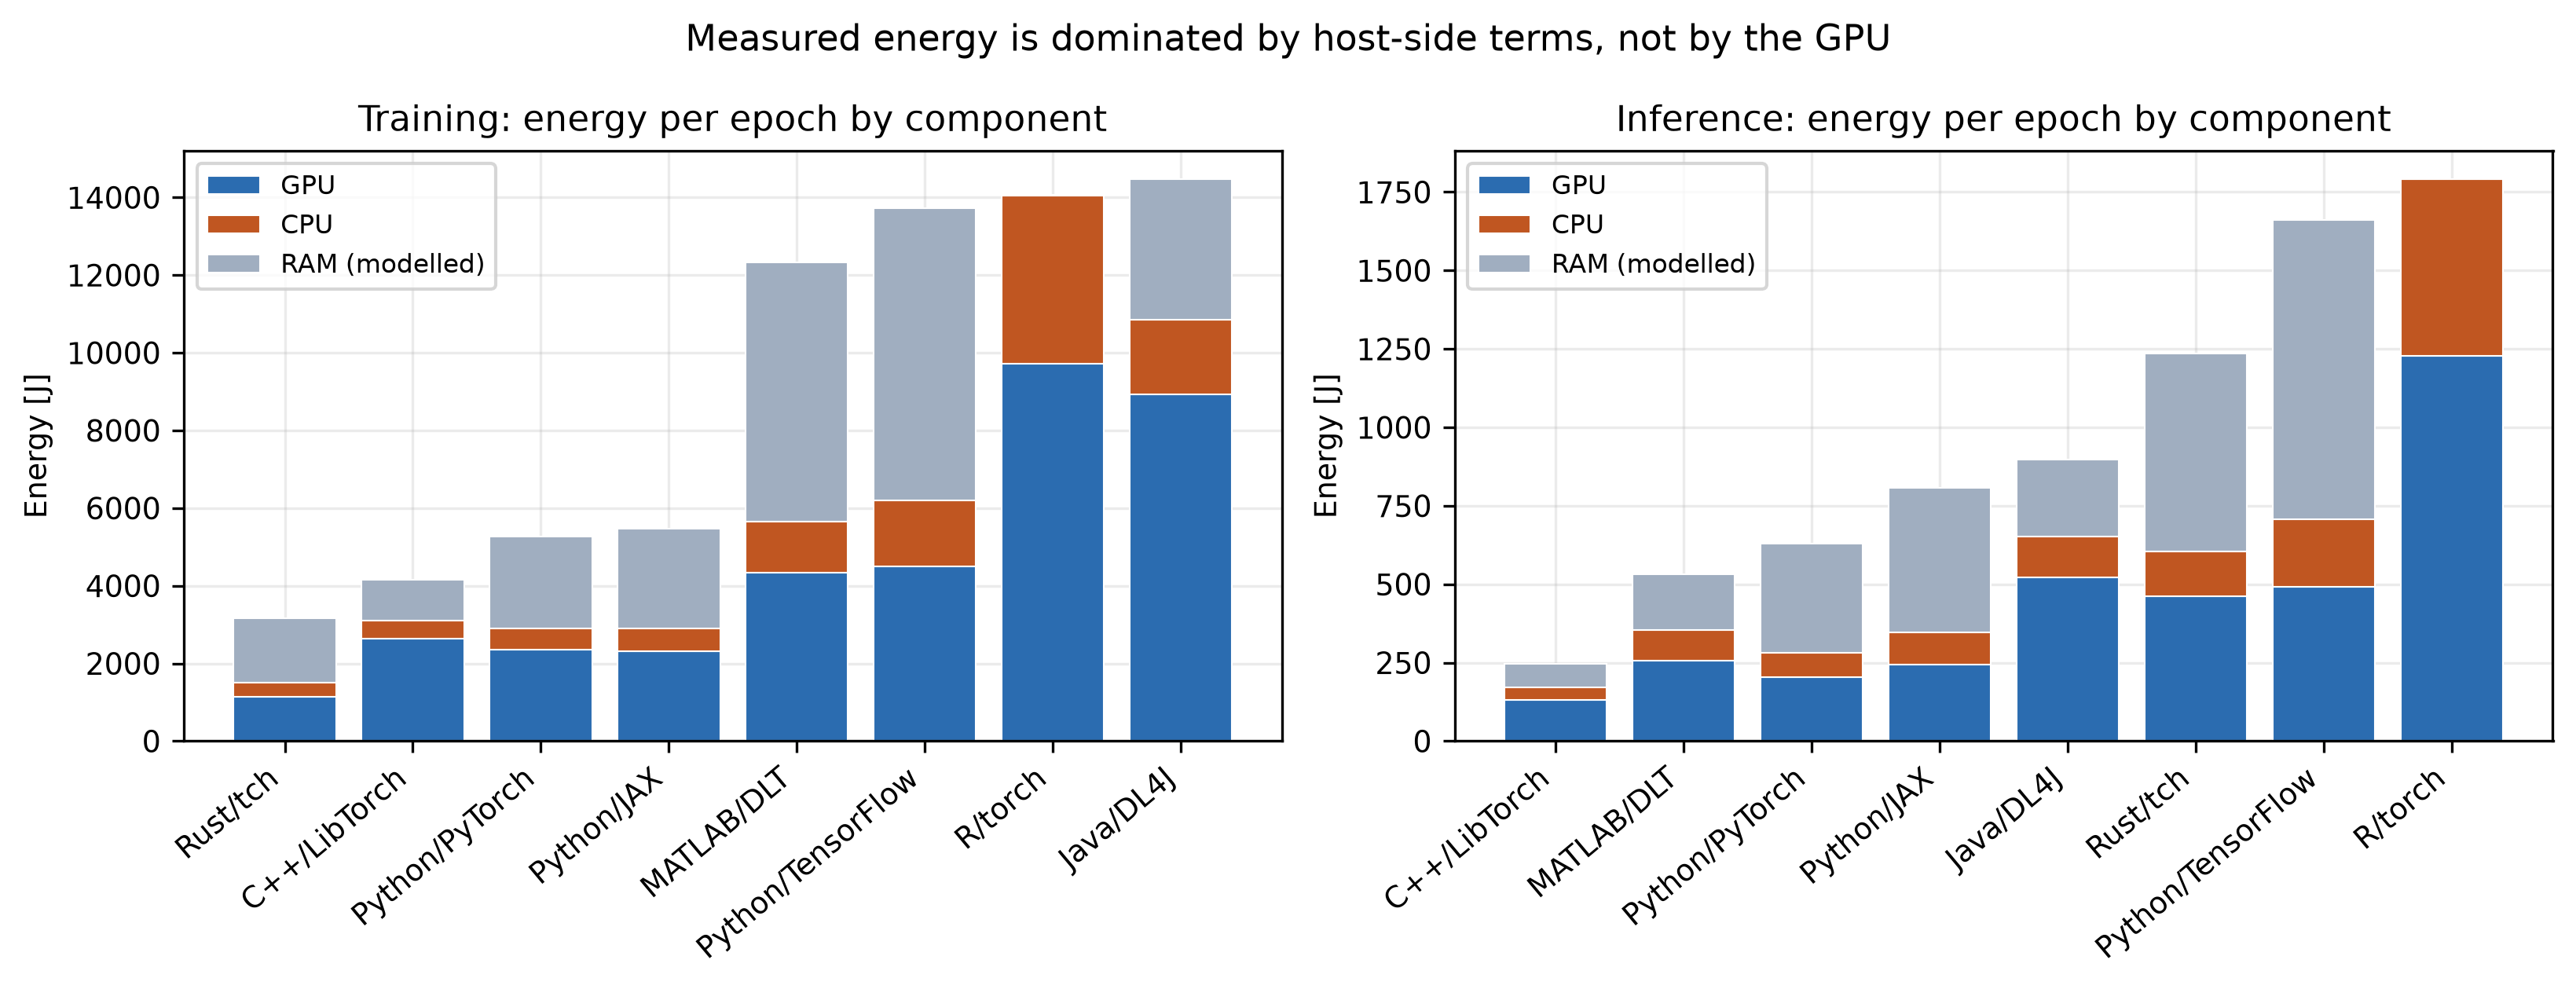
\includegraphics[width=\linewidth]{figures/fig_component_breakdown.png}
\caption{Energy per epoch split into GPU, CPU and modelled RAM. The RAM term is
not measured: for the CodeCarbon 2.8.x stacks it is a constant
\SI{188.84}{\watt} derived from \emph{installed} memory, so it grows only with
wall-clock time. It is the largest single component for four of the eight
ecosystems.}
\label{fig:components}
\end{figure}

\subsection{The workload does not load the accelerator}

Mean GPU power derived from the energy counter ranges from \SI{83}{\watt} to
\SI{197}{\watt} against a \SI{350}{\watt} board limit, and never approaches the
limit in any configuration. Between \SI{30}{\percent} and \SI{69}{\percent} of
the measured energy is GPU energy; the remainder is host-side. At that
utilisation the campaign measures data loading and dispatch more than it measures
deep learning (Figure~\ref{fig:gpuload}).

\begin{figure}[t]
\centering
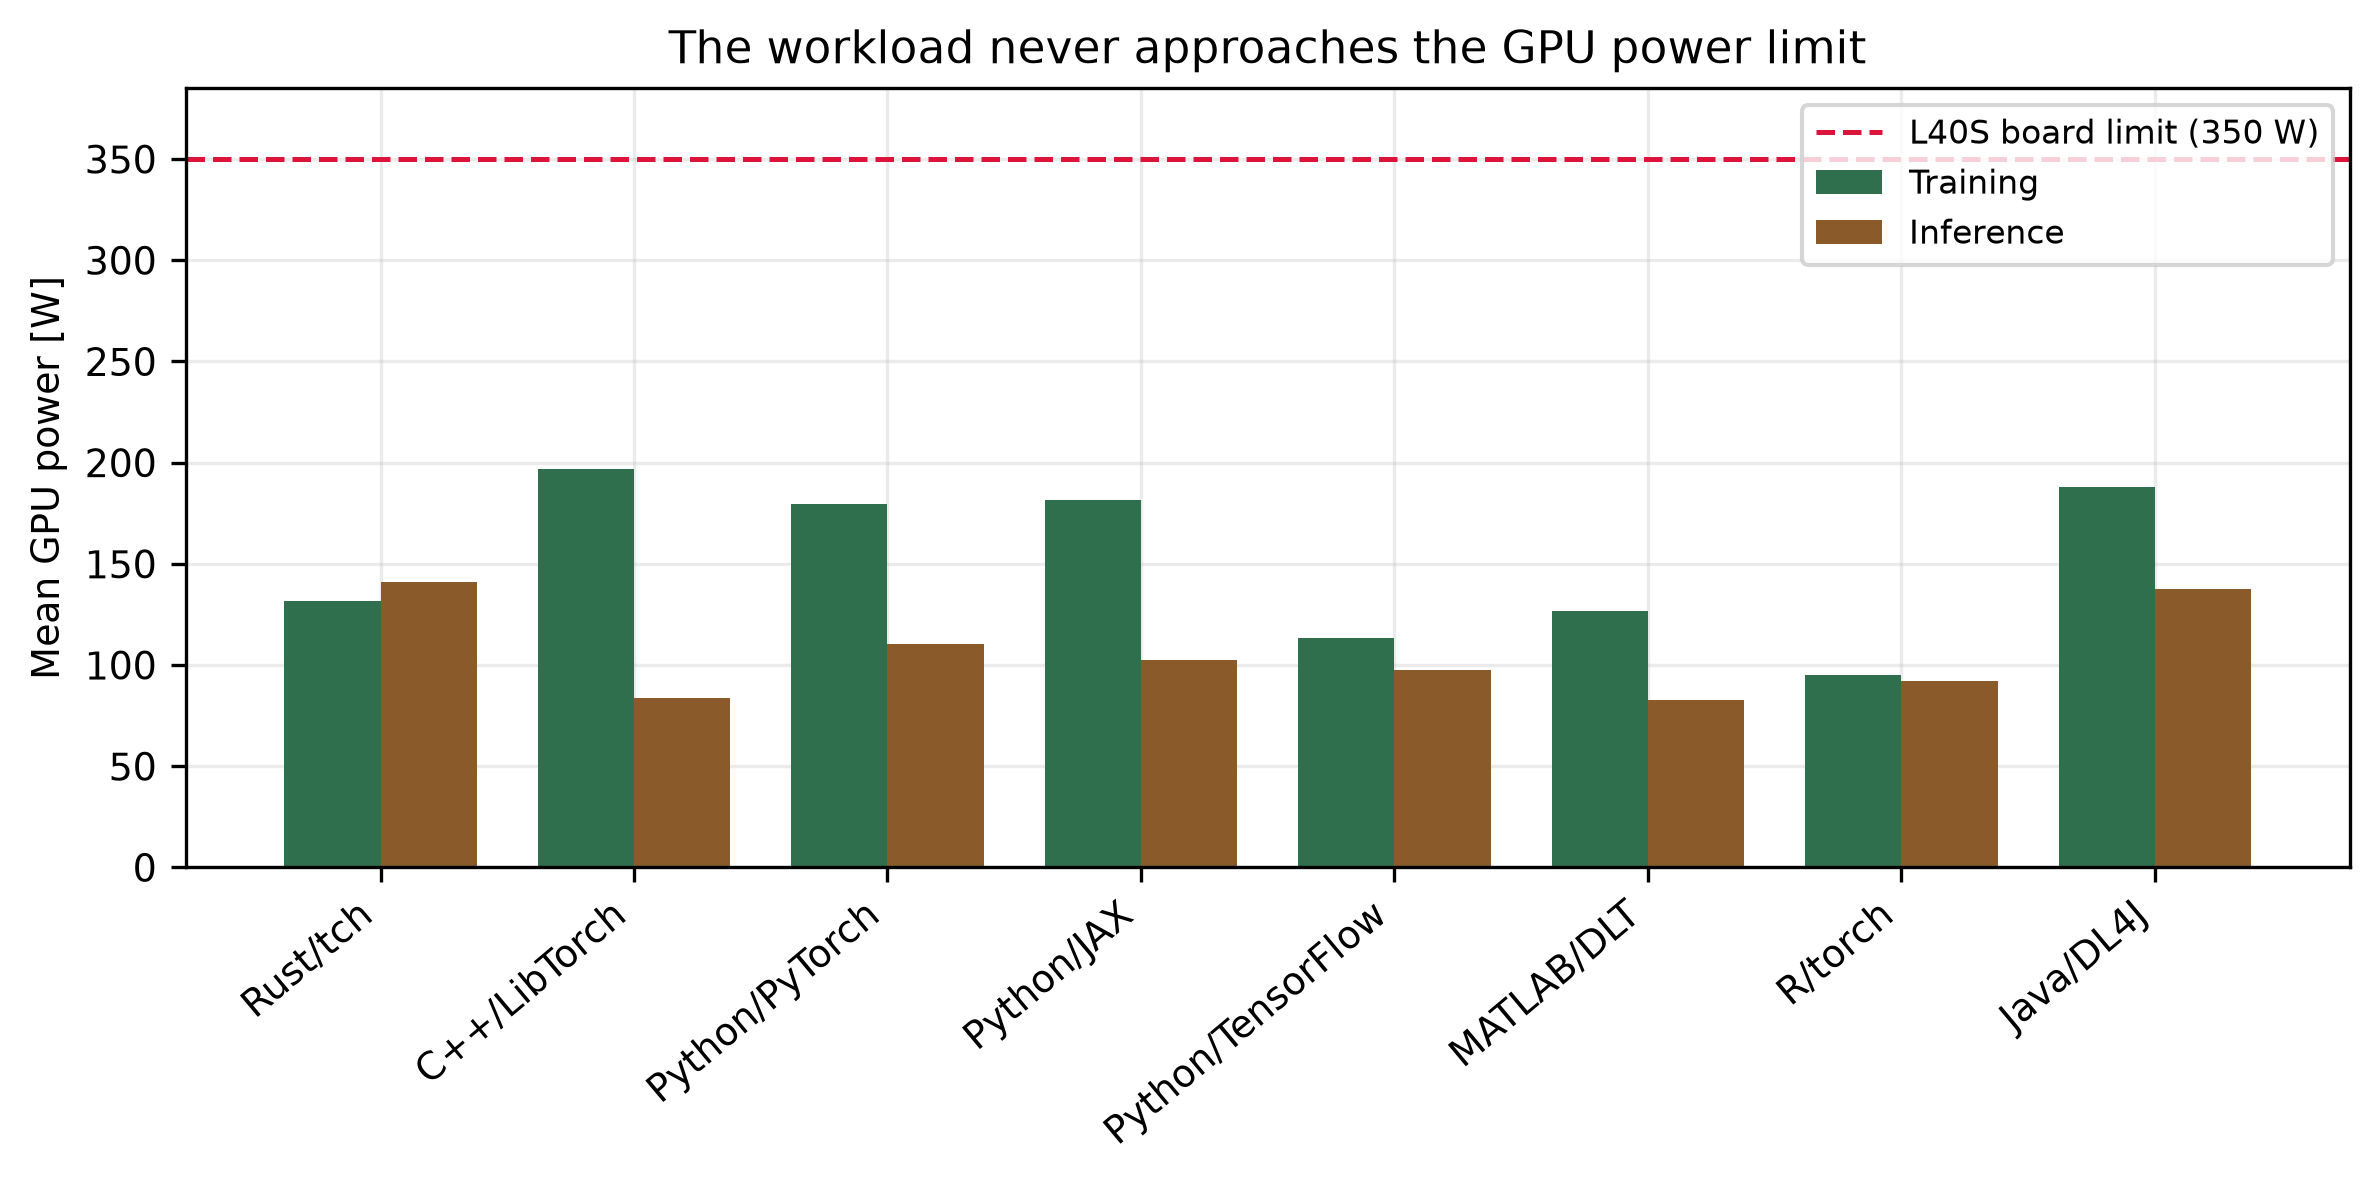
\includegraphics[width=0.72\linewidth]{figures/fig_gpu_load.png}
\caption{Mean GPU power per ecosystem and phase, against the board limit of the
measurement device. No configuration approaches the limit in either phase.}
\label{fig:gpuload}
\end{figure}

\section{The ecosystems did not run the same experiment}
\label{sec:implementation}

The manuscript states a common protocol: the same 30 epochs, learning rate,
optimiser and batch size. Reading the source of all eight implementations shows
otherwise.

\begin{table}[t]
\centering
\caption{Training protocol as implemented, read from source. The manuscript
states a common learning rate; two values are in use.}
\label{tab:protocol}
\small
\begin{tabular}{llrlrl}
\toprule
Ecosystem & Optimiser & LR & Loader mechanism & Threads & Input scaling \\
\midrule
Python/PyTorch    & Adam & 1e-4 & DataLoader workers & 2 & $[0,1]$ \\
Python/TensorFlow & Adam & \textbf{1e-3} & Keras generator & 1 & $[0,1]$ \\
Python/JAX        & Adam & 1e-4 & Keras generator & 1 & $[0,1]$ \\
C++/LibTorch      & Adam & 1e-4 & DataLoader workers & 2 & $[0,1]$ \\
Java/DL4J         & Adam & 1e-4 & AsyncDataSetIterator & 2 & $[0,1]$ \\
R/torch           & Adam & 1e-4 & dataloader workers & \textbf{0} & $[0,1]$ \\
Rust/tch          & Adam & \textbf{1e-3} & rayon, all cores & \textbf{96} & \textbf{mean/std} \\
MATLAB/DLT        & adam & 1e-4 & augmentedImageDatastore & 1 & $[0,1]$ \\
\bottomrule
\end{tabular}
\end{table}

\subsection{Data-loader parallelism, not language, tracks the ranking}

The largest single difference is how many CPU threads decode and feed images: from
zero (R decodes on the main thread) to all 96 cores (Rust, through \code{rayon}).
Spearman correlation between loader threads and mean epoch duration is
\(\rho=-0.73\) (\(p=0.04\)) across the eight ecosystems. The fastest stack
decodes on 96 cores; the slowest uses no loader workers; they differ by
\(11.6\times\) in duration.

Combined with the GPU-load result of Section~\ref{sec:instrument} --- the
accelerator at a fraction of its limit, duration accounting for essentially the
whole log energy spread --- the most parsimonious reading of the headline result
is that it ranks data-pipeline configurations.

\subsection{One ecosystem was not solving the same task}

Three defects in the Rust implementation all push in the direction of the
reported result:

\begin{itemize}\itemsep2pt
  \item \textbf{Fashion-MNIST was trained at \(28\times28\times1\).} The loader
        applied no resize and no channel replication, so training ran on the
        native grayscale image while \emph{its own evaluation loop} --- and every
        other ecosystem, in both phases --- used \(32\times32\times3\). The
        \code{conv1} input volume during training was \(0.26\times\) everyone
        else's.
  \item \textbf{Tiny ImageNet was trained at its native \(64\times64\)} in the
        ResNet binary, while the VGG binary passed \code{Some(32)} and every
        other ecosystem used \(32\times32\): four times the spatial work for the
        same nominal configuration, inside one ecosystem.
  \item \textbf{Evaluation ran one image at a time} (\code{iter\_batches(1)}) in
        all six binaries, against batch 128 elsewhere. Batch-1 GPU inference is
        launch-overhead bound.
\end{itemize}

The published numbers line up with the defects. Against the median of the other
stacks, this ecosystem's training energy is \(0.07\times\) for
ResNet-18/Fashion-MNIST --- the cheapest cell in the entire campaign, and
precisely the cell with the smallest input --- rising to \(0.61\times\); its
inference energy is \(1.51\)--\(1.95\times\) on CIFAR-100 and Fashion-MNIST.

The manuscript's \emph{training/inference ranking reversal}, reported as a
finding, is therefore reproducible for this ecosystem as a pure artefact of input
shape and evaluation batching.

\subsection{One ecosystem evaluated in training mode}

The TensorFlow stack built its functional graph with
\code{backbone(inputs, training=True)}, pinning training-mode behaviour into the
graph. Batch normalisation then used the statistics of the current batch during
evaluation as well. Because the test split is served in class order, each
evaluation batch held a single class and normalisation ran against degenerate
per-class statistics: measured test accuracy was \SI{21}{\percent} against
\SI{83}{\percent} on train, and \SI{86}{\percent} once the flag was removed.

Two consequences. The accuracy this stack would have reported was meaningless ---
but accuracy was never written to disk, so nothing surfaced it. And its inference
phase was measuring a different computation from every other ecosystem, all of
which switch to evaluation mode.

\subsection{The dataset itself was ambiguous}

Fashion-MNIST class~0 is \code{T-shirt/top}. Used verbatim as a directory name it
creates a \emph{nested} directory, so \code{train/T-shirt/} holds a \code{top/}
subdirectory rather than images. Loaders then disagree about what the dataset
contains: \code{ImageFolder} and \code{flow\_from\_directory} walk recursively and
recover the \num{6000} images, a loader listing only direct children sees an empty
class, and a loader using \code{read\_dir} yields the subdirectory as an image
path. The same dataset directory is three different datasets depending on who
reads it.

\section{Re-analysis under a common measurement boundary}
\label{sec:reanalysis}

Because the instrument differed across stacks, we report every result under three
energy definitions:

\begin{description}\itemsep2pt
  \item[as measured] CodeCarbon's total, instrument-confounded;
  \item[GPU only] the NVML energy counter alone --- the same instrument
        everywhere, and the only quantity attributable to the deep learning
        computation;
  \item[harmonised] GPU counter plus a single uniform \SI{107}{\watt} host model
        applied to every ecosystem.
\end{description}

\subsection{The rankings are not robust to the boundary}

\begin{table}[t]
\centering
\caption{Best and worst ecosystem, and spread, under each energy definition. The
identity of the worst ecosystem in training changes with the definition.}
\label{tab:spreads}
\small
\begin{tabular}{lllr}
\toprule
Phase & Energy definition & Best / Worst & Spread \\
\midrule
Training & as measured    & Rust/tch / Java/DL4J & \(4.58\times\) \\
Training & GPU only       & Rust/tch / R/torch   & \(8.54\times\) \\
Training & harmonised     & Rust/tch / R/torch   & \(9.94\times\) \\
Training & execution time & Rust/tch / R/torch   & \(11.63\times\) \\
\midrule
Inference & as measured    & C++/LibTorch / R/torch & \(7.28\times\) \\
Inference & GPU only       & C++/LibTorch / R/torch & \(9.30\times\) \\
Inference & harmonised     & C++/LibTorch / R/torch & \(8.83\times\) \\
Inference & execution time & C++/LibTorch / R/torch & \(8.47\times\) \\
\bottomrule
\end{tabular}
\end{table}

The headline figures quoted in the campaign --- \(4.6\times\) for training,
\(7.3\times\) for inference --- are the as-measured spreads. Under a common
boundary they become \(9.9\times\) and \(8.8\times\), and the worst ecosystem in
training changes identity.

\subsection{``Faster is not greener'' does not survive}

The campaign concludes that execution time is an unreliable proxy for energy. We
quantify the relationship rather than reading it off qualitative quadrants.

Within an ecosystem, energy is very nearly a deterministic linear function of
wall-clock time: the median \(R^2\) of energy on duration is \num{0.98}. This is
expected once Section~\ref{sec:instrument} is taken into account.

Across ecosystems, agreement between the energy ranking and the time ranking is:

\begin{center}
\small
\begin{tabular}{llrr}
\toprule
Phase & Energy definition & Spearman \(\rho\) & Discordant pairs \\
\midrule
Inference & as measured & 0.90 & 3 of 28 \\
Inference & GPU only    & 0.98 & 1 of 28 \\
Inference & harmonised  & \textbf{1.00} & \textbf{0 of 28} \\
\midrule
Training  & as measured & 0.95 & 2 of 28 \\
Training  & GPU only    & 0.93 & 2 of 28 \\
Training  & harmonised  & \textbf{0.98} & \textbf{1 of 28} \\
\bottomrule
\end{tabular}
\end{center}

Under a harmonised boundary the disagreement vanishes entirely for inference and
reduces to a single pair in training. The specific examples the manuscript gives
are exactly the pairs that disappear once the host power model is held constant.

\begin{figure}[t]
\centering
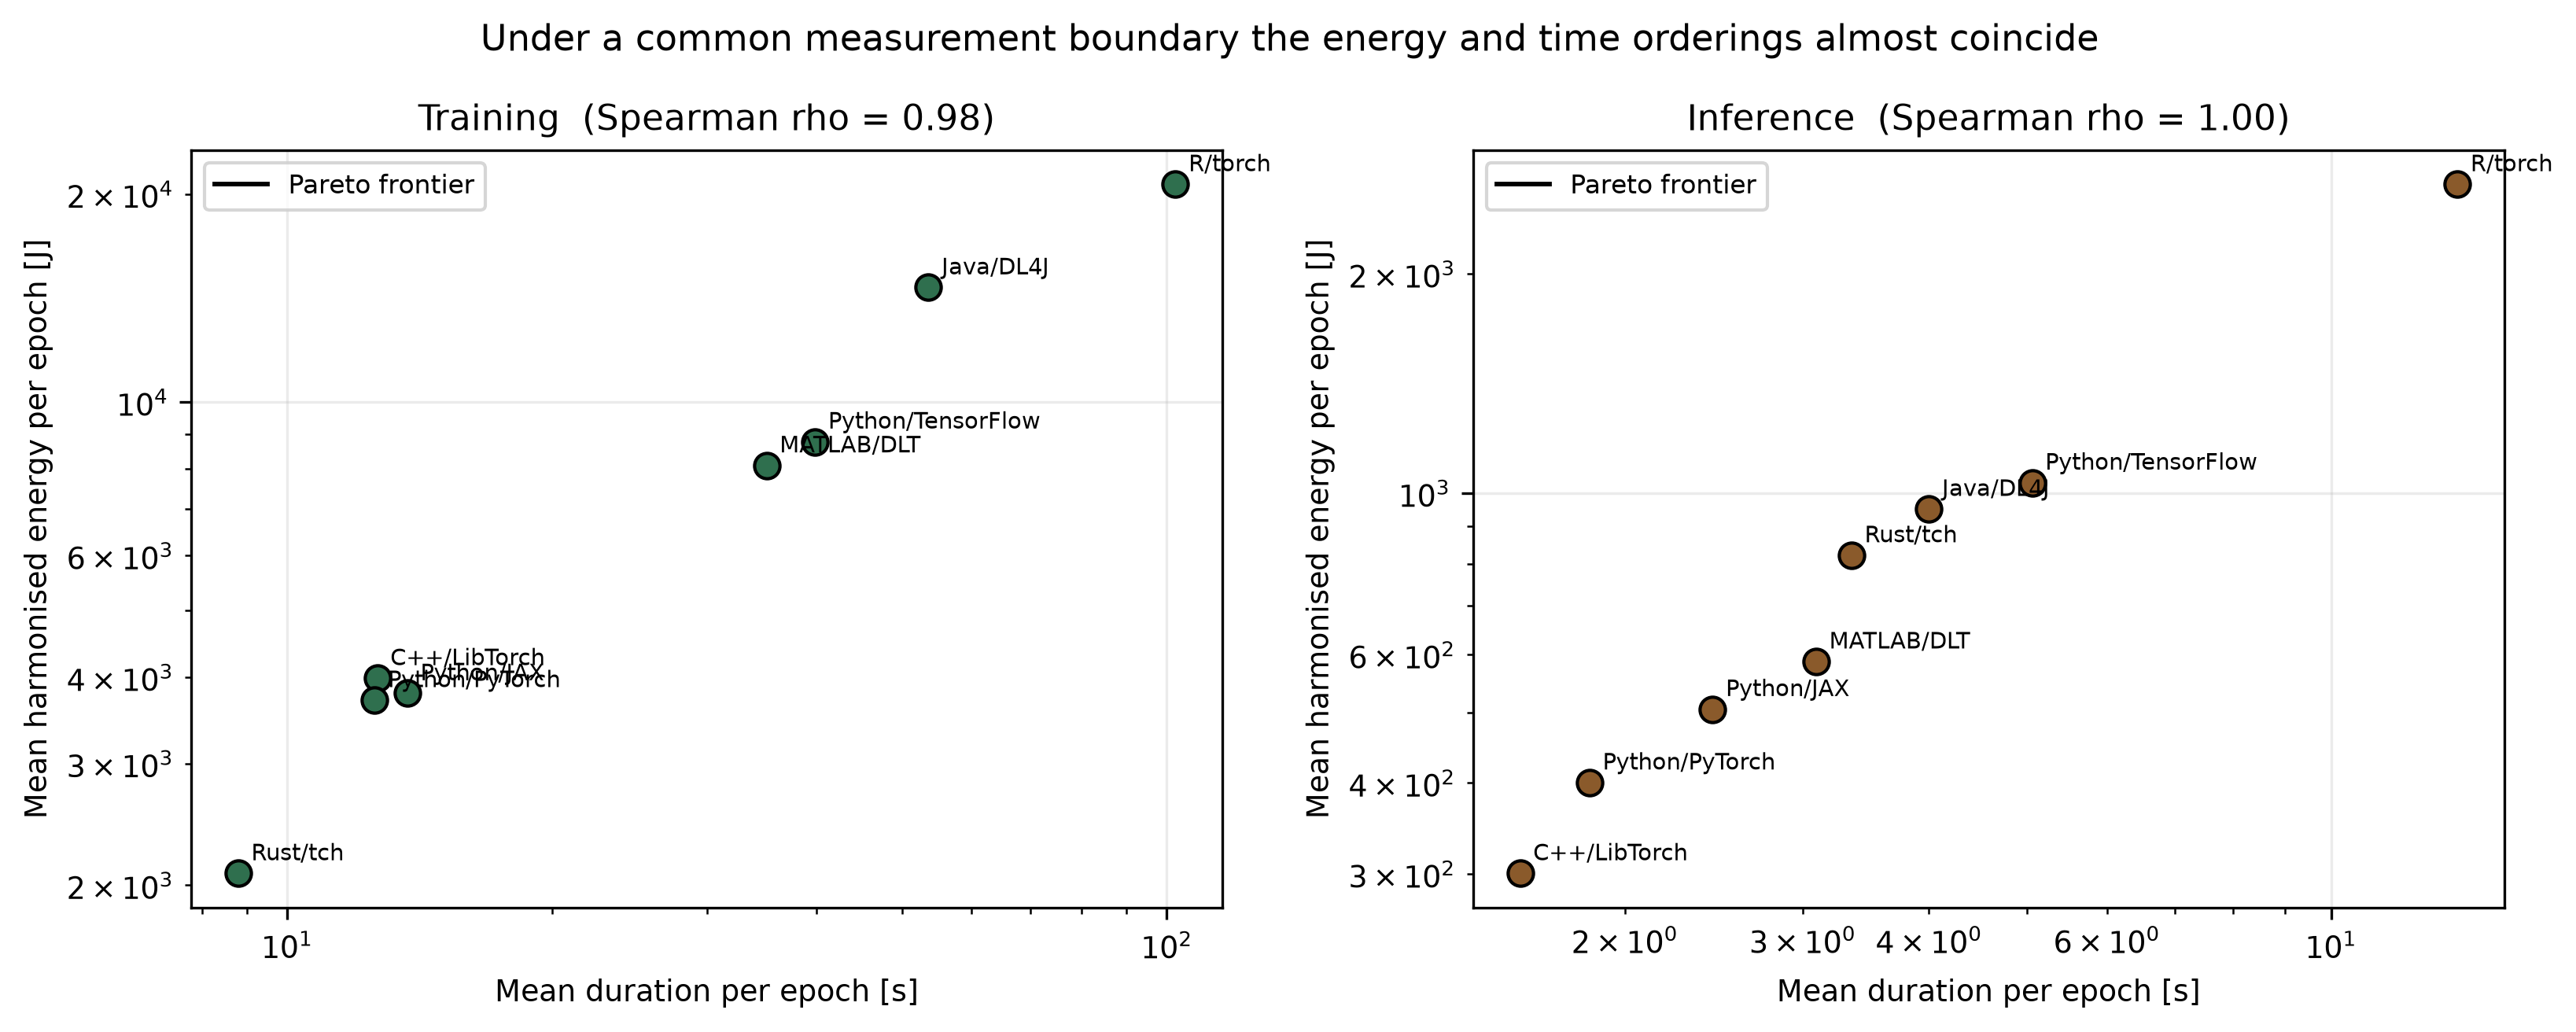
\includegraphics[width=\linewidth]{figures/fig_pareto.png}
\caption{Energy against duration per ecosystem under the harmonised boundary.
The orderings coincide for inference and differ by one pair in training; the
campaign's qualitative quadrant plot suggested a much weaker relationship.}
\label{fig:pareto}
\end{figure}

Decomposing energy as mean power times duration, \SI{98}{\percent} (inference) and
\SI{107}{\percent} (training) of the log spread is attributable to duration, with
a mean-power spread of only \(1.3\)--\(1.6\times\).

\subsection{The internal control group reproduces the whole effect}

Four of the eight ecosystems --- Python/PyTorch, C++/LibTorch, R/torch and
Rust/tch --- run the same LibTorch kernels. They are the study's natural control
group: any difference between them is binding, runtime and data-pipeline
overhead, not language.

Restricting the comparison to those four reproduces
\SIrange{98}{100}{\percent} of the full eight-stack spread on a log scale, in
every phase and under every energy definition. Whatever is being measured is
host-side.

We note that the group was not in fact controlled: the four stacks ran LibTorch
2.1.0, 2.5.x, 2.6.0 and 2.7.0 respectively --- six minor releases apart --- so
any difference between them also mixes in kernel, allocator and cuDNN changes.

\subsection{What the design can and cannot support}

Each of the 48 configurations was executed once, and the 30 epochs of a run are
repeated measurements of that run, sharing one initialisation, one JIT outcome,
one allocator state and one thermal trajectory. The effective number of
independent observations per configuration is one, not thirty.

We therefore report medians alongside means, bootstrap intervals over epochs
labelled explicitly as within-run dispersion, and effect sizes; and we do not
report a significance claim about ecosystems. Tests computed over epochs are
anti-conservative by an unknown factor: they compare the epochs of one run with
the epochs of another.

Separately, \num{158} rows (\SI{5.5}{\percent}) report a sampled GPU power of
\SI{0}{\watt} and \num{27} exceed the board limit, up to \SI{3054}{\watt}. These
are confined to CodeCarbon's \emph{sampled} power columns, which are unreliable
because \SI{69}{\percent} of the measured blocks are shorter than the
\SI{15}{\second} default sampling period. The energy columns come from the NVML
counter and show no such values.

\section{A catalogue of defect classes}
\label{sec:catalogue}

Table~\ref{tab:catalogue} collects the defects we found, each with a measured
effect. We report them as classes rather than as a list of bugs in one project:
every one of them is a plausible mistake in any study of this shape, and most are
invisible in the resulting data.

\begin{table}[t]
\centering
\caption{Defect classes, with the measured effect of each. ``Visible in the
data'' asks whether a reader given only the released measurements could detect
the problem.}
\label{tab:catalogue}
\small
\begin{tabular}{p{4.6cm}p{6.4cm}c}
\toprule
Class & Measured effect & Visible \\
\midrule
Unit mislabelling &
Energy reported in \si{\kilo\watt\hour} labelled as \si{\joule}; \(3.6\times10^6\) &
yes \\
\addlinespace
Mixed instrument versions &
\SI{231}{\watt} vs \SI{107}{\watt} of modelled host power; up to \SI{70}{\percent} of reported energy &
no \\
\addlinespace
Mixed tracking mode &
One stack at \SI{31}{\percent} host share against \(\sim\)\SI{50}{\percent} &
no \\
\addlinespace
Interpreter resolved from \code{PATH} &
CodeCarbon version becomes a property of the shell &
no \\
\addlinespace
Unsynchronised tracker &
Inference \SI{0}{\joule} recorded; training underestimated \SI{24}{\percent} &
no \\
\addlinespace
Divergent hyperparameters &
Two learning rates across eight stacks &
no \\
\addlinespace
Divergent loader parallelism &
0 to 96 threads; \(\rho=-0.73\) with duration, \(11.6\times\) spread &
no \\
\addlinespace
Divergent input shape &
One stack at \(0.26\times\) the \code{conv1} input volume; \(0.07\times\) energy &
no \\
\addlinespace
Divergent evaluation batching &
Batch 1 vs 128; \(1.5\)--\(1.95\times\) inference energy &
no \\
\addlinespace
Evaluation in training mode &
Test accuracy \SI{21}{\percent} vs \SI{86}{\percent}; different computation measured &
no\(^\dagger\) \\
\addlinespace
Silent CPU fallback &
Whole workload on CPU after a CUDA wheel mismatch; one warning line &
no \\
\addlinespace
Linker drops the CUDA dependency &
Same source, same LibTorch: \code{Cpu} vs \code{Cuda(0)} &
no \\
\addlinespace
Ambiguous dataset layout &
A class name containing \code{/} yields three different datasets &
no \\
\addlinespace
Host not idle &
Whole-machine tracking counts unrelated downloads and builds &
no \\
\bottomrule
\end{tabular}

\vspace{2pt}
\raggedright\footnotesize
\(^\dagger\) invisible because no ecosystem wrote its accuracy to disk; visible
the moment one does.
\end{table}

Two observations. First, only one of the fourteen is visible from the released
data --- the one that changes no conclusion. Second, several are not mistakes of
carelessness but defaults: the linker's \code{--as-needed} behaviour, CodeCarbon's
fallback power constants, a framework resolving CUDA wheels that do not match its
build. A study can be executed carefully and still land on all of them.

This is our argument for enforcement rather than discipline. The defects that
matter are the ones that produce plausible numbers, and plausible numbers are
exactly what review cannot catch.

\section{Making the comparison possible}
\label{sec:infrastructure}

The defects in Sections~\ref{sec:instrument} and~\ref{sec:implementation} share a
shape: each is a place where seven independent implementations were free to
differ, and did. Our response is to remove the freedom where it is not part of
the research question, and to make the remaining differences fail loudly.

\subsection{A written specification}

We state the experiment once, as a document rather than as folklore: model
source, optimisation, data pipeline, backend, measurement and replication.
Anything the specification does not pin is a documented degree of freedom, and
anything it pins is checkable.

\subsection{One measurement bridge and one run contract}

The five per-stack CodeCarbon bridges are replaced by one. Every ecosystem drives
it through a line protocol (\code{START}, \code{STOP}, \code{METRIC},
\code{EXIT}), all of which are synchronous, and reads its parameters from a
shared environment contract: output directory, ecosystem, model, dataset,
repetition, seed, epoch count, data and model roots, and the interpreter to
measure with.

Environment variables rather than command-line flags: adding argument parsing to
a C++ binary, a Maven target, an \code{Rscript} and a Rust binary is four
different pieces of plumbing, and four places for the stacks to drift apart
again.

Two things the contract makes impossible rather than merely discouraged. The
interpreter is named explicitly, so no stack can silently be measured by whatever
\code{python3} the shell resolves. And the harness refuses to start when the
framework cannot see the accelerator, so a CPU fallback aborts the run instead of
being recorded as an ecosystem property.

\subsection{One model where the backend allows it}

For the stacks that share LibTorch, the model is exported once as TorchScript
from \code{torchvision} and loaded by each binding. Verified end to end: all six
modules load into Rust and take an optimiser step through the variable store,
with parameter counts matching the Python export exactly
(\num{11227812} for ResNet-18/CIFAR-100), and all six load and forward in R.

R is a documented exception. In \code{torch} 0.17.0 a script module's
\code{\$train()} and \code{\$eval()} raise \code{unused argument}, and the
underlying handle is not reachable through the object's documented fields, so a
loaded module cannot be switched between training and evaluation. Since the
shared modules are exported in training mode, this stack would evaluate with
batch normalisation using batch statistics --- exactly the TensorFlow defect of
Section~\ref{sec:implementation}. It therefore builds its own model, and the
architecture parity that holds for Python, C++ and Rust does not hold for R.
That is a property of the binding, and it belongs in the threats to validity
rather than being papered over.

\subsection{An automated conformance checker}

The specification is enforced by a checker that reads the source the campaign
actually runs: 56 checks covering learning rate, batch size, loader threads, input
scaling, evaluation batching, shared-module use, backend version alignment,
bridge use, tracker synchronisation, device assertion and the absence of
hard-coded paths.

The checker is the piece we would keep if we could keep only one. It turns
``the stacks should be configured the same'' from an intention into a claim that
fails when it stops being true.

\subsection{Every ecosystem verified on the accelerator}

All seven in-scope ecosystems now run on the GPU under the shared contract and
write per-epoch accuracy. Getting there required per-stack fixes that no
documentation mentions: the linker must be told to keep \code{torch\_cuda} or the
Rust binary silently runs on the CPU; \code{CUDA::nvToolsExt} must be defined
before \code{find\_package(Torch)} because NVTX left the CUDA toolkit in CUDA 12;
the C++ embedded interpreter resolves \code{site-packages} from whichever
libpython it was linked against rather than from the campaign environment; R's
\code{liblantern.so} links against \code{libcudart.so.12} while the R bundle ships
it under a hashed name; and DL4J 1.0.0-M2.1 links against the CUDA 11.6 runtime
and is the last release of that API, so on a CUDA 12 host the backend fails with
\code{libcudart.so.11.0: cannot open shared object file} and ND4J reports only
``no backend on your classpath''.

\begin{table}[t]
\centering
\caption{Test accuracy after one epoch on CIFAR-100, identical settings and seed.
The first campaign could not perform this check: no ecosystem wrote its accuracy
to disk.}
\label{tab:convergence}
\small
\begin{tabular}{lrr}
\toprule
Ecosystem & Test accuracy & Train loss \\
\midrule
Python/PyTorch & \SI{19.84}{\percent} & 3.828 \\
C++/LibTorch   & \SI{20.01}{\percent} & 3.822 \\
Rust/tch       & \SI{20.62}{\percent} & 3.798 \\
R/torch        & \SI{20.79}{\percent} & 3.687 \\
Java/DL4J      & \SI{17.14}{\percent} & 3.784 \\
\bottomrule
\end{tabular}
\end{table}

Table~\ref{tab:convergence} is the check that matters. Five independent
implementations agree within \SI{3.6}{\percent}, and the four sharing the
LibTorch backend agree within one point. Java sits lower, which is consistent
with it building its own graph rather than loading the shared module --- and
that is now something a reader can see rather than something nobody recorded.

\section{Threats to validity and what remains}
\label{sec:threats}

\paragraph{We do not report a corrected ranking.}
The corrected infrastructure exists and every ecosystem has been verified on the
accelerator, but the replicated campaign has not been executed at the time of
writing. We consider this the honest position: a ranking produced before the
defects of Sections~\ref{sec:instrument} and~\ref{sec:implementation} are fixed
would inherit them, and a ranking produced after them is a different experiment
that deserves its own reporting.

\paragraph{Residual confounds we could not remove.}
Two survive by construction rather than by oversight. DL4J 1.0.0-M2.1 links
against the CUDA 11.6 runtime and is the last release of its API, so the Java
ecosystem cannot be brought onto the CUDA 12 toolchain the other six use; the
stack now carries its own redistributables, which makes it reproducible but does
not remove the version difference. And the R binding cannot switch a script
module between training and evaluation, so it cannot share the traced model.
Both are properties of the ecosystems, and arguably part of what one is measuring
when one measures an ecosystem --- but they are not the binding overhead the
study set out to isolate.

\paragraph{The workload.}
The campaign runs the accelerator at \SIrange{24}{56}{\percent} of its power
limit, so it measures data loading and dispatch more than deep learning. A
replicated campaign should add at least one configuration that saturates the
accelerator, and report utilisation alongside energy so a reader can see which
regime a result belongs to.

\paragraph{The instrument itself.}
We now read hardware counters directly ---
\code{nvmlDeviceGetTotalEnergyConsumption} for the accelerator and Intel RAPL for
the CPU package --- and run CodeCarbon over the same window as a cross-check.

It is worth being precise about what was wrong with the original instrument,
because it was not accuracy. Measured on the replication machine with both
instruments bracketing the same window, CodeCarbon 3.3.0 agrees with the counters
to within \SI{1}{\percent} for block durations from \SI{2}{\second} to
\SI{40}{\second}, for GPU and CPU alike. The failure mode is that it
\emph{substitutes a model when a counter is unavailable, and says so only in a
log line}: where RAPL cannot be read the CPU term becomes a constant, the RAM term
is derived from installed memory rather than from use, and the model changed
between major versions. An instrument that refused to run would have been
preferable to one that quietly estimated.

This matters for how a number should be reported. NVML plus RAPL is a
\emph{chip-level} boundary: it excludes the power supply, fans and drives that a
wall meter would see. Published validations place software estimators within tens
of percent of a wall meter, so a chip-boundary figure must not be presented as a
whole-system one. The figure the campaign under audit reports sits between the two
boundaries and corresponds to neither --- for four ecosystems roughly two thirds
of it was a model of RAM power derived from how much memory the machine happened
to have installed.

We had no wall meter, and say so rather than implying a boundary we did not
measure.

\paragraph{Generalisation.}
Everything here concerns one campaign, one hardware platform and one model class.
The defect \emph{classes} of Section~\ref{sec:catalogue} are, we believe, general
to studies of this shape; the effect sizes are not.

\paragraph{Our own errors.}
Two of the defects in Section~\ref{sec:catalogue} we introduced ourselves while
repairing the study, and caught only because the accuracy check of
Table~\ref{tab:convergence} existed: switching the Rust stack to the shared
TorchScript module made it evaluate in training mode, costing 15 accuracy points,
because \code{TrainableCModule} ignores the training flag passed to
\code{forward\_t}. We measured contaminated blocks ourselves by running package
downloads while the campaign was tracking whole-machine energy. We report this
because it is the argument of the paper in miniature: the defects that matter are
the ones that produce plausible numbers, and the only reliable defence is a check
that fails.


\section{Related work}
\label{sec:related}

Cross-language energy comparisons and cross-framework deep learning comparisons
are both established. Georgiou et al. compare PyTorch and TensorFlow with
statistical tests, effect sizes, comparable accuracy across frameworks and
function-level profiling, and report that the energy ranking of deep learning
frameworks reverses between training and inference. Alizadeh and Castor measure
the energy and inference time of deep learning runtime infrastructures across
frameworks and execution providers, and report that efficiency is hard to predict
and is driven by GPU and CPU usage. Cross-language studies at the level of
general-purpose benchmarks likewise report that faster execution does not imply
lower energy.

Our contribution is orthogonal to these. We do not add another ranking; we ask
what has to be true of an experimental apparatus before any such ranking means
anything, and we show --- on a real campaign, with measured effect sizes --- how
far an apparatus can drift while producing entirely plausible numbers. The
phase-reversal result is a useful illustration: we reproduce it for one ecosystem
as a pure artefact of evaluation batching and input shape
(Section~\ref{sec:implementation}).

\section{Conclusion}
\label{sec:conclusion}

The question of whether language--framework ecosystems differ in energy cost
remains open, and we think it is worth answering. What we can say is that the
apparatus needed to answer it is more demanding than it appears.

In the campaign we audited, the instrument was configured five different ways,
the workload differed between stacks in learning rate, input shape, evaluation
batching and loader parallelism, and two stacks could have been running on the
CPU without any recorded evidence either way. Each of these produces plausible
numbers. Together they produce a plausible story --- one that does not survive a
common measurement boundary.

The practical lesson is that a cross-ecosystem energy study needs a written
specification and a mechanism that enforces it, in the same way that a
performance benchmark needs a warm-up policy. We provide both, and the checker is
the part we would keep if we could keep only one thing: it is what turns
``the stacks should be configured the same'' into a claim that fails loudly when
it stops being true.

\end{document}
